\chapter{Reactor Mass Model} \label{ch:mass_model}
The reactor mass model was created as a submodel of the power cycle mass
model. The reactor mass model was designed to take flow property inputs (T, P,
$\dot{m}$) and constrain a reactor concept that is both coolable, and critical
after 10 years of full power operation. The reactor model was developed in
Python. The attribute of interest is the mass of
the valid concept, but other useful values such as geometry, fuel fraction,
and fluid-flow paramters are available from the solver. Before the mass model
could be built, some important design decisions needed to be made.

\section{Initial Design Constraints}
    In order to develop a reactor mass model, the concept was constrained with
some general design decisions. The chosen design needed to be simple and robust.
The simplest reactor fuel concept is block fuel with coolant channels. 
Block fuel is a common design choice for space reactors that operate at relatively 
low power and burnup compared to power reactors. Two fuel types were chosen; one for
near-term and the other for long-term technological readiness options. Uranium
oxide was chosen as the near-term fuel option for its high melting temperature.
UMo and UN fuel were not considered because of tempearture limitations, despite
their thermal conductivity and uranium density advantages. Inconel-718 was
chosen as cladding for its high temperature strength and corrosion
compatability with sCO$_2$. With these design choices, the reactor mass model
could be developed from first principle heat transfer and fluid flow equations
coupled with a critical core radius constraint.

\subsection{Fuel Composition}
Two reactor fuels were considered for modeling. The near term technical
readiness choice was 93\% enriched \uox. The advanced fuel option investigated
was 93\% enriched uranium-tungsten cermet (UW). UW-cermet fuel is UN fuel suspended in a
tungsten matrix. UW-cermet fuel has been considered for nuclear thermal
propulsion due to its high thermal conductivity and resistance to fuel swelling.
While a relatively unusual fuel form, NASA has conducted research to prove the 
manufacturability of UW-CERMET cores for nuclear thermal propulsion applications\citep{hickman_fabrication_2005}.
The tradeoff with UW-CERMET fuel is a reduced uranium density, 60\% of the fuel
volume is UN, 40\% is tungsten. As shown below in Table \ref{tab:uox_comp} and
Table \ref{tab:uw_comp}, the \uox fuel has a significantly higher uranium
density than the UW-CERMET fuel.

\begin{table}[h]
  \centering
  \caption{\uox fuel composition}
  \begin{tabular}{cc}
    \toprule
    Isotope   & Mass Fraction [-] \\
    \midrule
     8016     & 0.1520 \\
    92235     & 0.7886 \\
    92238     & 0.0594 \\
  \end{tabular}
  \label{tab:uox_comp}
\end{table}
    
\begin{table}[h]
  \centering
  \caption{UW-CERMET fuel composition}
  \begin{tabular}{cc}
    \toprule
    Isotope   & Mass Fraction [-] \\
    \midrule
     7015     &  0.0260 \\
     74180    &  0.0006 \\ 
     74182    &  0.1396 \\
     74183    &  0.0758 \\
     74184    &  0.1632 \\
     74186    &  0.1531 \\
     92235    &  0.4107 \\
     92238    &  0.0309 \\
  \end{tabular}
  \label{tab:uw_comp}
\end{table}

\newpage

\subsection{Fuel Design Modularity}
A fuel design was chosen to constrain the reactor model. In order to support
alternate designs, the reactor model was developed in a modular fashion.
Different fuel configurations such as pin-type or TRISO particle fuel could be
explored with a different set of heat transfer equations and criticality models.
This will be discussed in more detail in following sections.

\section{Thermal Hydraulic Theory}
    The first considered constraint of a valid reactor design was coolability. The reactor must
not melt and the integrity of the fuel must be maintained for the duration of
the mission. To ensure the thermal hydraulic validity of a chosen design, 
    1D heat transfer and bulk-averaged fluid flow calculations were performed. The 1D
heat transfer and fluid equations were coupled with analytical flux shape
factors from nuclear engineering literature to determine the maximum extractable
thermal power for each reactor design. A 1D resistance network is used to
determine the maximum thermal generation for a given core design and temperature
drop between fuel meat and coolant. An iterative solving scheme was developed to
converge the heat transfer and fluid flow equations.

\subsection{Flow Properties}
All flow properties were axially averaged between their inlet and outlet values.
The inlet and outlet flow conditions, thermal power, and mass flow rate are
dictated by the power cycle configuration and requirements. Property tables for
both CO2 and H2O coolants as a function of pressure and temperature were 
generated using EES and interpolated using SciPy's 2D interpolation functions
\citep{scipy}, \citep{EES_citation}.
The interpolated properties included: thermal conductivity [W/m-K], density
[kg/m$^3$], viscosity [kg/m-s], and specific heat [J/kg-K].

\subsection{Core Geometry}

Important core geometry parameters were calculated. The coolant flow area,
average distance of conduction in the fuel, volume fraction of cladding in
coolant, number of coolant channels, convection surface area, LD, and the cross
sectional area for conduction in the fuel. The core radius is set by a critical
radius constraint dependent on the fuel fraction. This will be discussed in a
later section.

Fuel area and volume is derived from the core radius and fuel fraction. Where
$AR$ is the core aspect ratio.

\begin{equation}
    A_{fuel} = frac_{fuel}*r_{core}^2*\pi
\end{equation}
\begin{equation}
    V_{fuel} = A_{cool}*AR*r_{core}
\end{equation}

The fraction of cladding in the coolant is derived from the coolant channel
radius and cladding thickness.

\begin{equation}
    frac_{clad} = \frac{(r_{channel} + t_{clad})^2 - r_{channel}^2}{r_{channel}^2} 
\end{equation}

In a similar vein, coolant flow area is derived from the core radius, cladding
fraction, and fuel fraction

\begin{equation}
    A_{cool} = (1-frac_{fuel})*(1-frac_{clad})*r_{core}^2*\pi
\end{equation}

\begin{equation}
    V_{cool} = A_{cool}*AR*r_{core}
\end{equation}

The number of coolant channels is derived from the area of each channel and the
core flow area.

\begin{equation}
    N_{channels} = \frac{A_{cool}}{(r_{channel} + t_{clad})^2 * \pi}
\end{equation}

The convection surface area is dervied from the channel radius, core length, and
number of channels.

\begin{equation}
    A_{conv} = 2*r_{channel}*\pi*r_{core}*AR*N_{channels}    
\end{equation}

The length over diameter is derived from the channel radius and core length.

\begin{equation}
    LD = \frac{r_{core}*AR}{2*r_{channel}}
\end{equation}

The average distance to conduction is derived from fuel area and number of
channels.

\begin{equation}
    R_{cond} = \frac{\sqrt{\frac{A_{fuel}}{N_{channels}}}}{2}
    \label{r_cond}
\end{equation}

The cross sectional area for conduction in the fuel was conservatively estimated
as the convection surface area. In reality, the cross-sectional area changes as
heat transfers from the center of the fuel meat to the coolant channels.


These are the important equations defining the 1D geometry for a coolable
reactor. Once the geometry has been defined, the flow conditions are modeled.

\subsection{Flow Equations}

Once the core geometry has been defined, the flow is characterized using
bulk-averaged flow conditions and the reactor geometry. The mass flux, coolant
velocity, Reynold's number, Nusselt number and average heat transfer
coefficients are calculated.

Mass flux is derived from flow area and the mass flow rate dictated by the power
cycle. Flow velocity can be calculate from mass flux and density.

\begin{equation}
    \dot{G} = \frac{\dot{m}}{A_{flow}}
\end{equation}

\begin{equation}
    v = \frac{\dot{G}}{\rho}
\end{equation}

The Reynold's number is derived from flow velocity, density, viscosity, and the
characteristic flow length (channel diameter, D).

\begin{equation}
    Re = \frac{\rho v D}{\mu}
\end{equation}

The Nusselt number is calculated using the same correlations as EES. Laminar,
turbulent, and transitional flows are all treated differently.

The average heat transfer coefficient is derived from the Nusselt number and
thermal conductivity of the fluid.

\begin{equation}
    \bar{h} = \frac{Nu k_{cool}}{D}
\end{equation}

\subsection{1D Thermal Generation Modeling}

With a fully defined geometry and fully characterized flow, the maximum thermal
output of the core is calculated. The maximum generation (at the center of the
core) is calculated using a 1D resistance network. The three resistances in the
network are: conduction in the fuel, conduction in the clad, and convection from
the clad to the coolant. Gap and interface resistances were ignored.

Resistance to conduction in the fuel was approximated as plane wall conduction.
\begin{equation}
    R_{fuel} =  \frac{R_{cond}}{k_{fuel}A_{cond}}
\end{equation}

\begin{equation}
    R_{clad} = log(1+\frac{t_{clad}}{r_{channel}})
\end{equation}

\begin{equation}
    R_{conv} = \frac{1}{2\bar{h}r_{channel}L\pi N_{channels}}
\end{equation}

The maximum heat transfer rate at the fuel centerline was derived from the
resistance network and the temperature drop. The temperature drop was determined
by the maximum fuel temperature (estimated to be half the melting temperature of
the fuel) and the bulk coolant temperature.

\begin{equation}
    Q^{'''}_{max} = \frac{dT}{R_{fuel} + R_{clad} + R_{conv}}
\end{equation}

Finally, the thermal generation at fuel centerline is scaled by the axial and
radial flux profiles to account for the cosine and bessel function shapes of the
flux. The scaling factor was taken from El-Wakil's Nuclear Heat Transport
\citep{heat_trans_wakil}.

\begin{equation}
    Q_{gen} = Q^{'''}_{max} * 0.275
\end{equation}

\subsection{1D Thermal Hydraulic Calcuations}

    The governing equations above describe a coolable
reactor design. A Python code was written to solve the system of equations
defining the geometry, flow conditions, and 1D heat transfer in the reactor. The
code utilizes Scipy's optimization package. The 'optimize\_scalar' function is
used to guess fuel fraction values. For each fuel fraction, the above equations
are used to determine $Q_{gen}$, an error exists between $Q_{gen}$ and the
required thermal reactor output dictated by the power cycle requirements. The
optimization function minimizes the squared difference between $Q_{gen}$ and the
thermal power requirements. When the solver converges on a fuel fraction, the
code returns a coolable reactor design. Since the core radius was set by a
critical radius constraint, this reactor is also neutronically valid for the
duration of the 10 year mission.

    The thermal hydrauilc code also calculates the mass of each reactor. This
mass includes fuel, cladding, coolant, reflector material and the pressure
vessel. The pressure vessel thickness was calculated as a function of pressure
and outer core radius (including the reflector) for stainless steel at \~700K
using an ASME vessel thickness standard. Equation \ref{eq:pv_thick} was used to
define the pressure vessel thickness. This correlation is a conservative
estimate for pressure vessels and is adequate to ensure the integrity of the
vessel.

\begin{equation}
    T_{vessel} = \frac{RP}{S + 0.6P}
    \label{eq:pv_thick}
\end{equation}

\section{Reactor Mass Modeling Results}
The results of the reactor mass model are hard to analyze outside the context of
the overall power cycle optimization. In the most general sense, the reactor
mass model can be described as:

\begin{equation}
    m_{reactor} = f(\dot{m}, T_{in}, T_{out}, P_{in}, P_{out})
\end{equation}

The reactor is dependent on flow conditions, and configuration. Further
complicating the analysis, the flow conditions are coupled by the power cycle
efficiency.

\section{Input Dependence}

\subsection{Mass Flow Rate}
The mass flow rate through the core is dictated by the power cycle model. It is
the free variable used by the power cycle model to meet the required 40 kWe
output of the system. Increasing the mass flow rate improves the heat transfer
coefficient from the fuel to the coolant. Reactors with higher mass flow rates
have less resistance to convection and better cooling. While the mass flow rate
helps heat transfer in the reactor, it is also used to adjust power output. For
a fixed coolant temperature rise, increasing the mass flow rate increases the
required thermal output of the reactor. Increasing the output of the core always
increases the mass. Mass flow rate is a tradeoff between heat transfer
performance and required thermal power.

\subsection{Coolant Temperature}
Bulk coolant temperatures were used to calculate coolant properties and the
temperature drop from the fuel to coolant. Increasing the coolant temperture
decreases the temperture drop. This decrease in $\delta$T reduces the
coolability of the core, requiring a larger core volume to deliver the same
thermal power. While increasing coolant temperature reduces the thermal power
density of the reactor, it also improves the efficiency of the power cycle. A
more efficient cycle requires a smaller thermal input to generate a fixed amount
of electrical power.

\subsection{Coolant Pressure}
Bulk coolant pressures were used to calculate coolant properties. Pressure also
impacts the thickness of the pressure vessel. Higher pressure systems require a
thicker pressure vessel for containment.

\subsection{Thermal Power}
During the mass model development, reactor response to thermal power was the
metric to analyze changes in the model. The reactor mass is most strongly
dependent on thermal power. Core power density limits require larger reactor
masses for higher powers. A fixed coolant flow rate of 1 [kg/s] was used to test
the mass model. As mentioned previously, this is not a realistic test for the
reactor response since the mass flow rate of the coolant tends to increase with
increasing thermal power. Nevertheless, thermal power for fixed flow inputs was
used to test the mass model outside the context of the power cycle model. Figure
\ref{fig:mass_vs_q_uo2_co2} shows the reactor mass dependence on the power
cycle.

\begin{figure}[h]
    \centering
    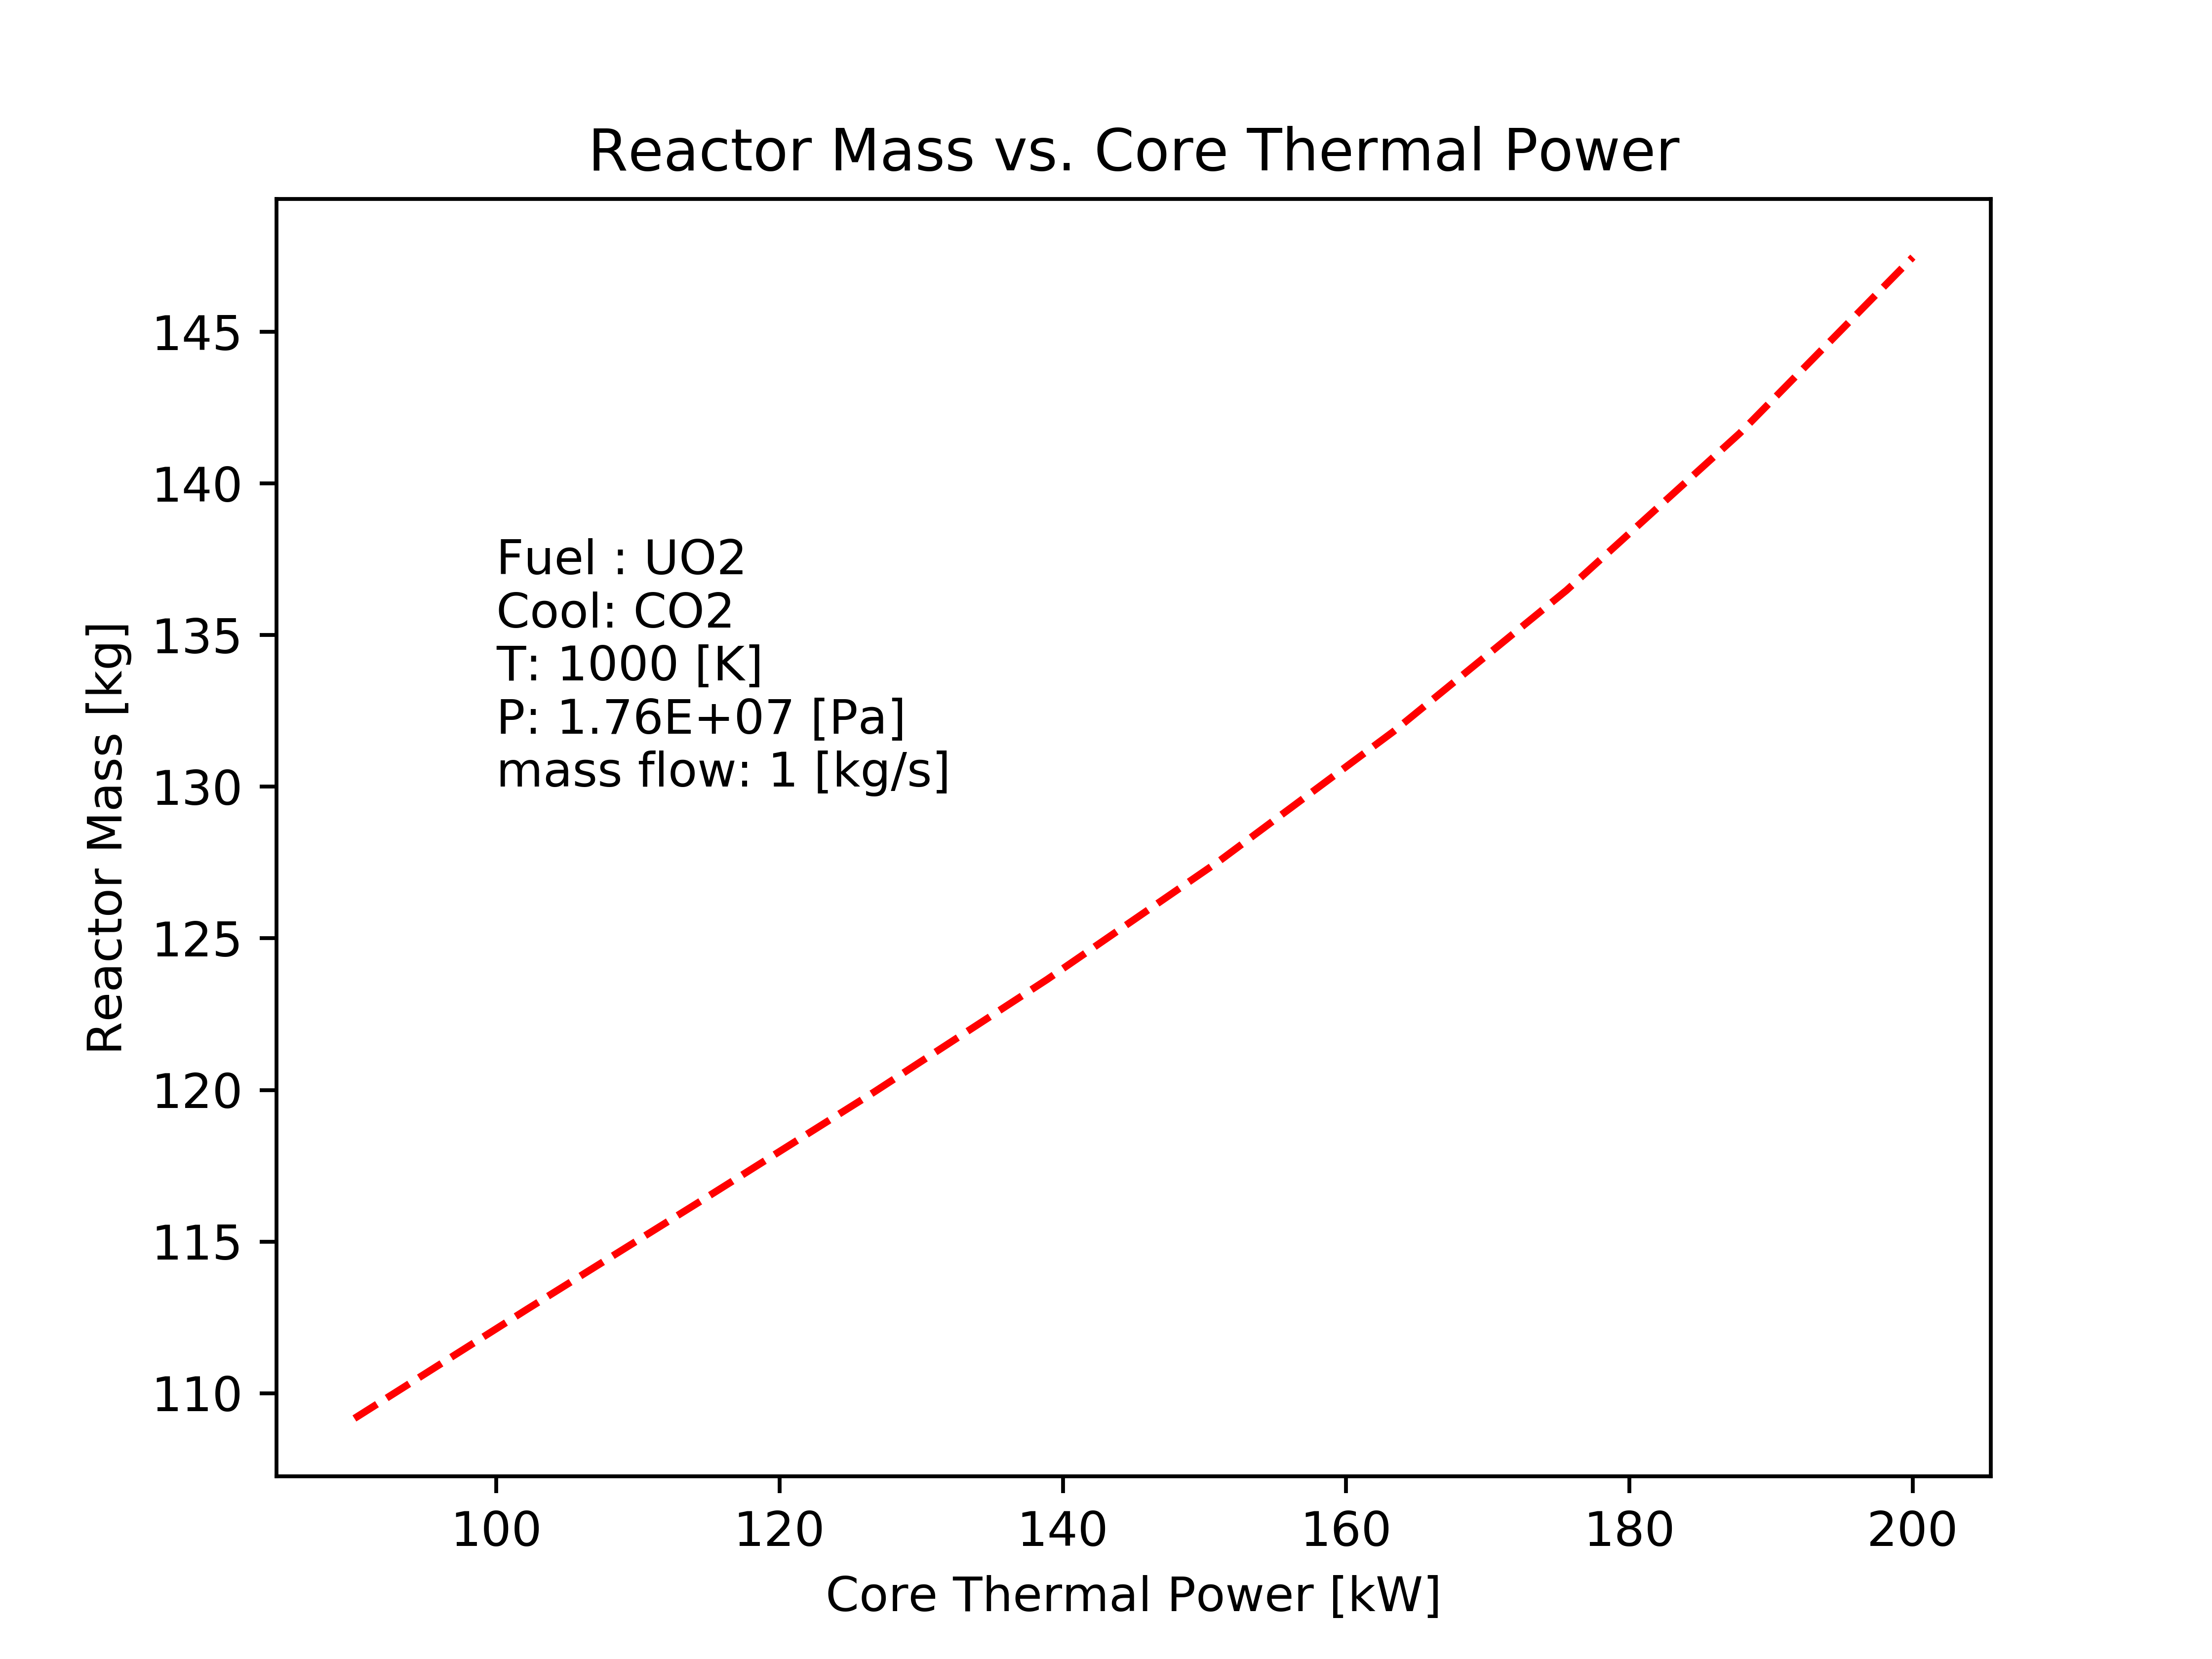
\includegraphics[width=4in]{../images/mass_vs_q_uo2_co2.png}
\caption{Reactor mass power dependence}
\label{fig:mass_vs_q_uo2_co2}
\end{figure}

\section{Conclusion}
A reactor mass model was developed from thermal hydraulic and reactivity
requirements (discussed in \ref{ch:critical_radius}). The model solved the heat
transfer equations iteratively to return a reactor model that meets the thermal
input requirements of the power cycle. The mass model was demonstrated here for
the \uox-\codiox  reactor configuration. Three other configurations were
considered using UN-\codiox, \uox-\water, and UN-\water. The results of these
configurations, as well as their corresponding reactivtiy models can be found in
Appendix \ref{ch:appendix-a}.
